\documentclass[Integrationstest/Integrationstest_main.tex]{subfiles}
\begin{document}

\lstdefinestyle{customc}{
    breaklines=true,
    language=C,
    showstringspaces=false,
}
\lstset{style=customc}

\section{Integrationstest mellem Playerside}
\subsection{Introduktion}
I dette afsnit beskrives intregationstesten mellem to Playersides og RPi'en. Her testes kommunikationen mellem Playerside og RPi, specifikt at alle protokol beskeder kan modtages og sendes korrekt. Til testningen bruges en tidlig udgave af RPiAppen. 
\subsection{Integrationstest mellem Playerside og RPiApp}
For at teste kommunikationen, skal vi simulere beskeder fra BallDispenser og Webpage: Indsættelse af mønt og modtagelse af data fra Webserver. Når systemet starter udsender RPi'en beskeden 'IDLE' til begge Playersides. Derefter simuleres indsættelse af en mønt, hvor RPi udsender beskeden 'STARTING'. Her vil begge Playersides sende beskeden "0x3F" = alle kopper er placeret. Normalt vil systemet først gå i stadiet "PLAYING" indtil data er modtaget fra WebPage, men dette simuleres i GameController klassen. Nu sendes "PLAYING" til Playersides, hvor den ene Playerside sender "0x3F" og den anden "0x00" = Ingen kopper tilbage. Her vil GameController registrere at et hold har tabt (Ingen kopper tilbage), og derved sende stadiet "LOST" til den ene Playerside og "WON" til den anden. Beskederne bliver sendt hvert sekund, det kan således ikke defineres helt som asynkrone beskeder, og dette påvirker afviklingstiden.\\\\
Simulering af BallDispenseren og WebPage gøres via MsgQueue-systemet. Her sender GameController beskeder til sig selv, som normalt ville komme fra boundary klasserne: 
\begin{lstlisting}
//Simuler at boundary klassen BallDispenser har modtaget information om indsaettelse af moent
GameControllerMsgQueue_->send(BallDispenser::NEW_INFO, new BallDispenserResponse(&BallDispenserMessage.COIN_INSERTED));

//Simuler at WebPage har sendt information om brugeren og initiere PLAYING-stadiet. 
state = GAME_STATE_PLAYING;
GameControllerMsgQueue_->send(SYSTEM_STATE::PLAYING);
\end{lstlisting}
Koden er måske lidt uoverskuelig og forvirrende, men det vigtige element er at forstå at de simulerer møntindsættelse og initiering af PLAYING-stadiet. Desuden blev der lavet en ekstra constructor, som kun modtager en pointer til to PlayersideWrite objekter, da det ikke er nødvendigt at have BallDispenser, Display eller Webpage operationel. 
\newpage
\subsubsection{Testopstilling}
Til testning af kommunikationen blev der brugt to PSoC enheder og en RPi. Begge PSoC enheder er programmeret til at være en Playerside (Med adresseren 0x10 og 0x11). En Rasberry Pi Zero W bruges til at eksekvere RPiApp. Analog Discovery bruges til at måle alt som bliver sendt fra de forskellige enheder. 
\begin{figure}[H]
    \centering
    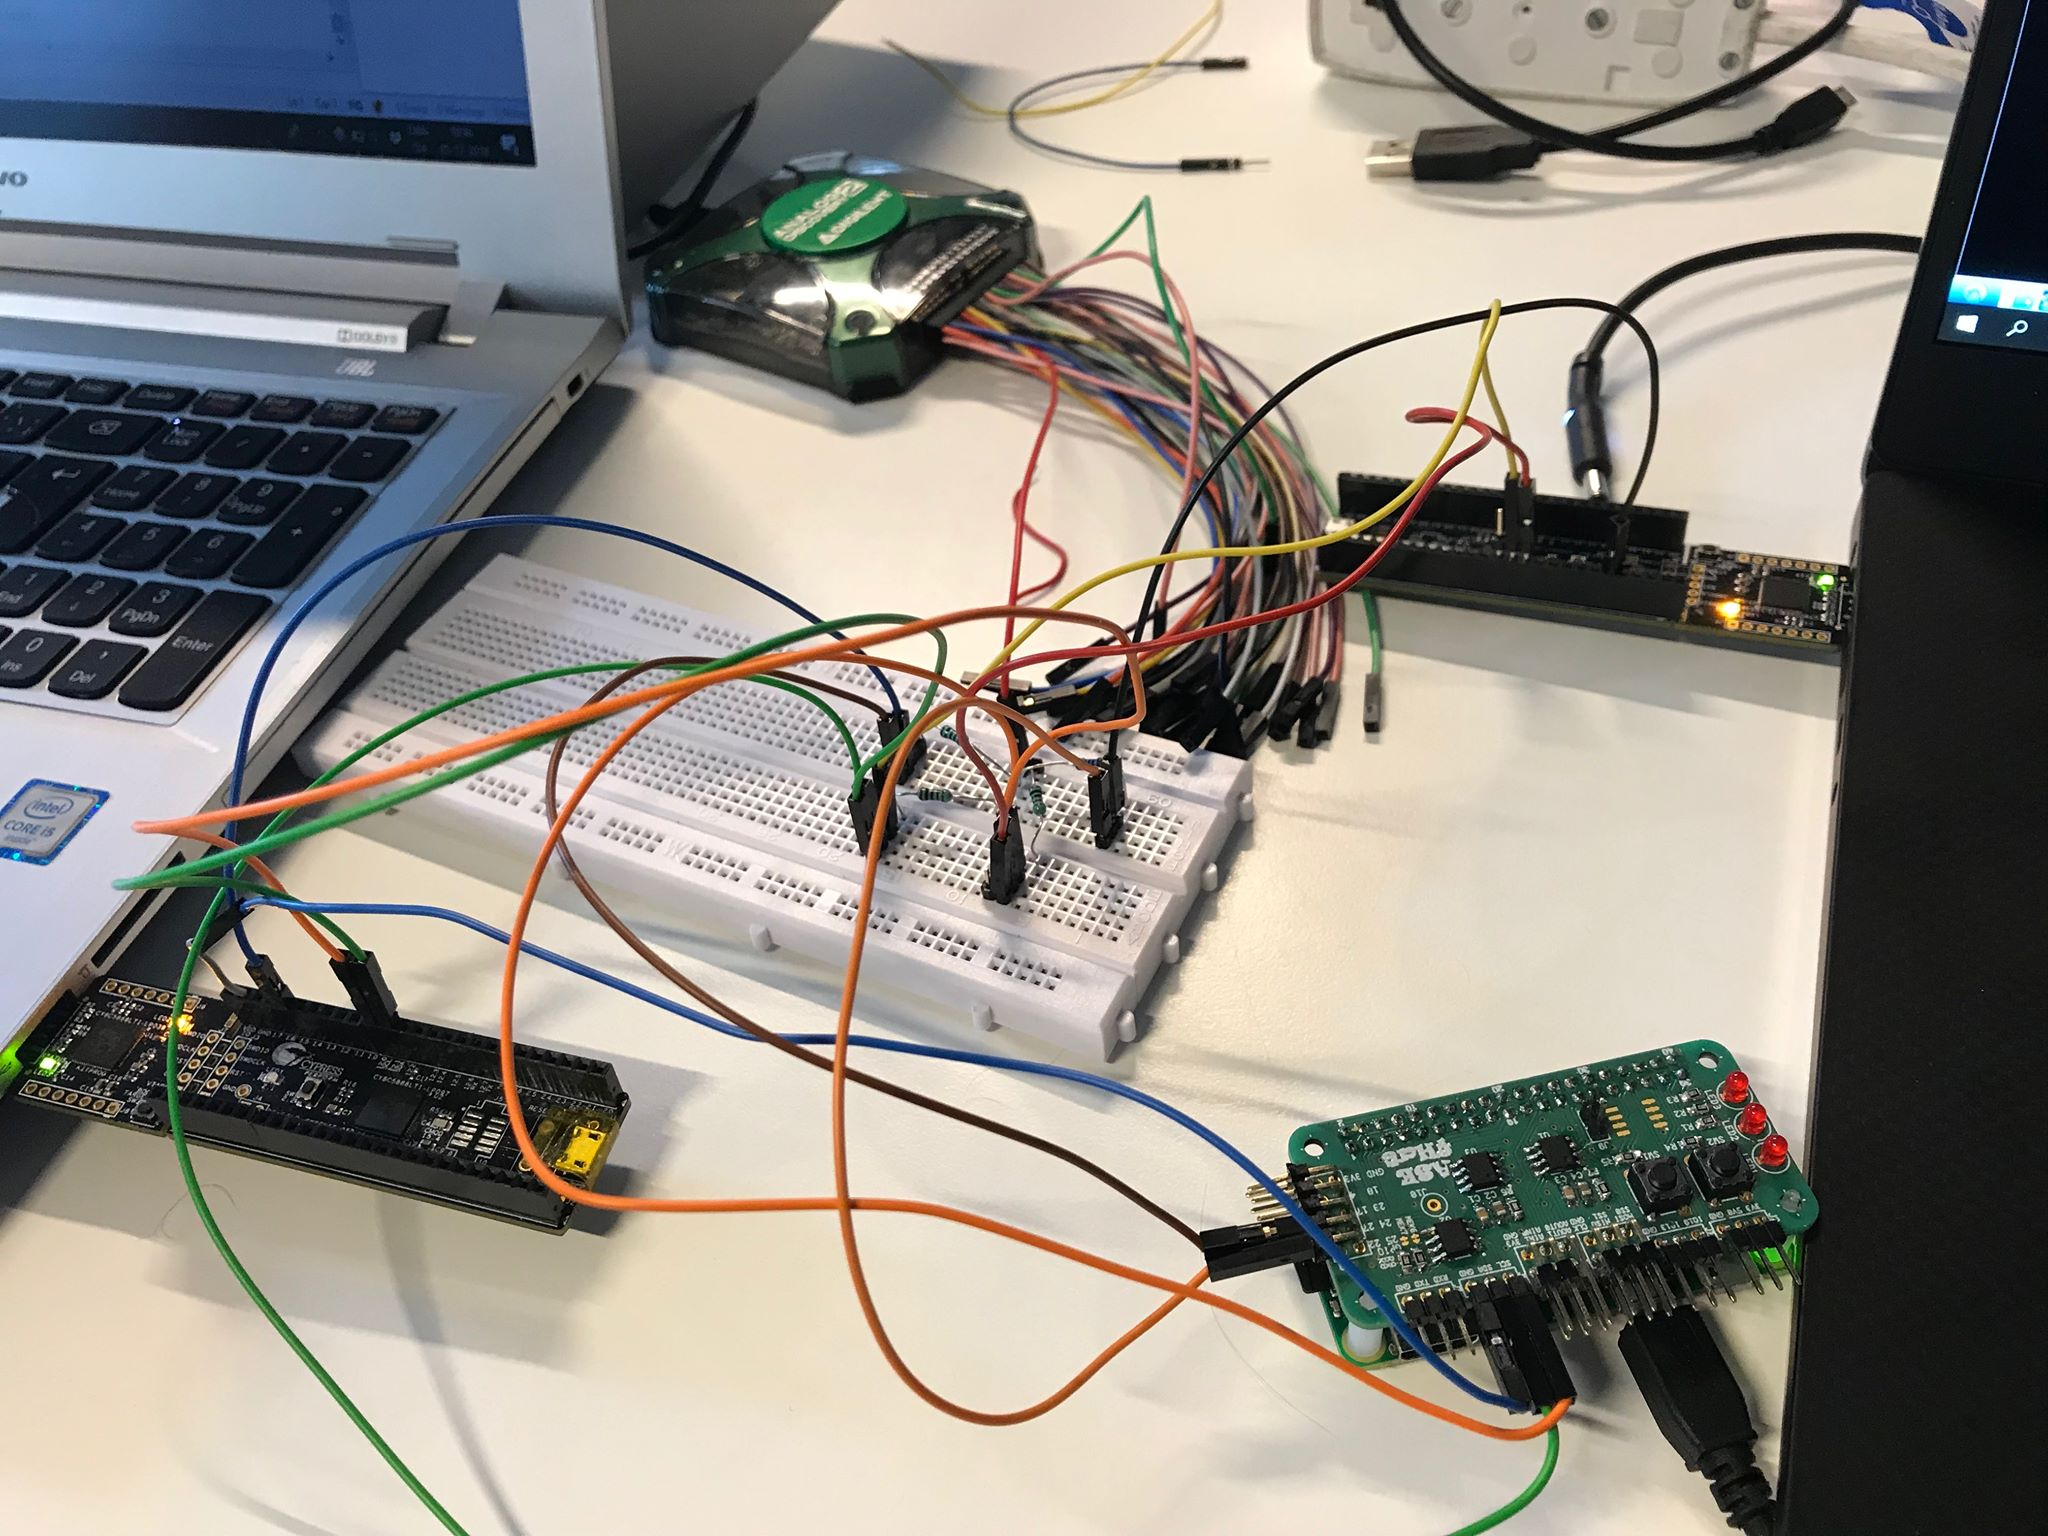
\includegraphics[width=1\textwidth]{Integrationstest/PlayersideogRPi/graphicsRPivPlay/integrationPlayervRPi.jpg}
    \caption{Testopstilling - 2 PSoC enheder og en RPi}
    \label{fig:test_Playerside_RPi}
\end{figure}

\subsubsection{Fremgangsmetoden for test}
\begin{enumerate}
    \item Indsæt kernemodulet "playerSide.ko" på RPi. 
    \item Indsæt overlayet "playerSide.dtbo" på RPi. 
    \item Afvikl ekseverbar fil i terminalen "test\_program". 
    \item Undersøg og dokumentér data sendt og modtaget fra RPi 
    \item Undersøg og dokumentér data sendt og modtaget fra Playerside 1 og 2. 
\end{enumerate}

\subsubsection{Resultater}
\begin{figure}[H]
    \centering
    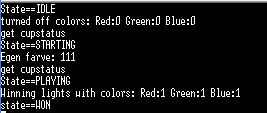
\includegraphics[width=1\textwidth]{Integrationstest/PlayersideogRPi/graphicsRPivPlay/Playerside1_teraterminal.png}
    \caption{Playerside 1 terminal}
    \label{fig:test_Playerside_terminal}
\end{figure}
\begin{figure}[H]
    \centering
    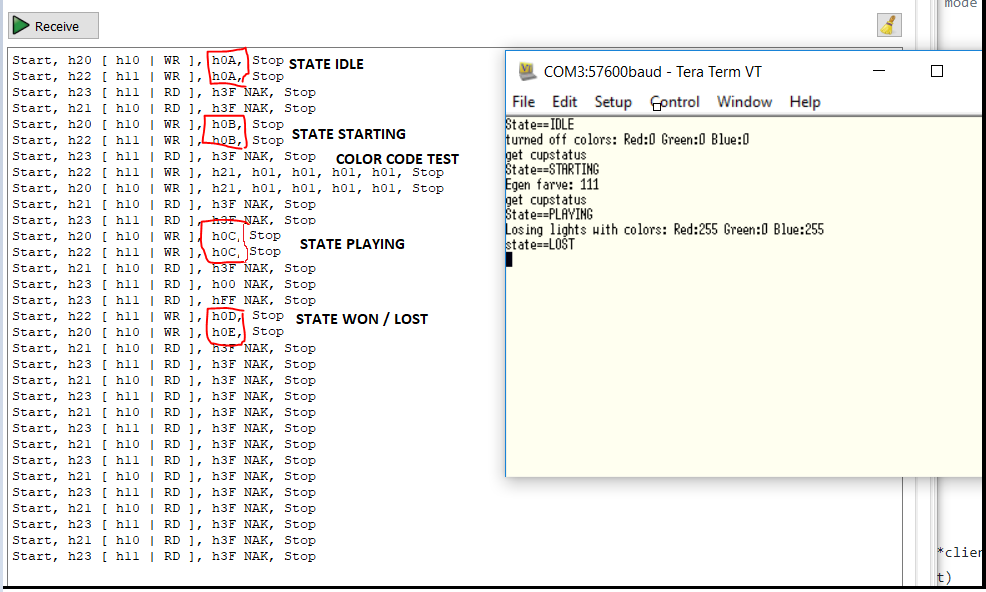
\includegraphics[width=1\textwidth]{Integrationstest/PlayersideogRPi/graphicsRPivPlay/Analogogterminal.png}
    \caption{Playerside 2 terminal, samt Analog Discovery målinger}
    \label{fig:test_Playerside_analog}
\end{figure}
Output fra RPi terminal: 
\begin{verbatim}
root@raspberrypi0-wifi:~# ./test_program
SYSTEM_STATE::IDLE
PS_WRITE1: STATE IDLE
PS_WRITE2: STATE IDLE
NEW_INFO : COIN_INSERTED
SYSTEM_STATE::STARTING
CUPS, PlAYING!
HandlePlayersideResonse
TEAM1: 111111
TEAM2: 111111
CUPS, PlAYING!
HandlePlayersideResonse
TEAM1: 111111
TEAM2: 111111
PS_WRITE1: STATE STARTING
PS_WRITE2: STATE STARTING
CUPS, PlAYING!
HandlePlayersideResonse
TEAM1: 111111
TEAM2: 111111
CUPS, PlAYING!
HandlePlayersideResonse
TEAM1: 111111
TEAM2: 111111
CUPS, PlAYING!
HandlePlayersideResonse
TEAM1: 111111
TEAM2: 111111
CUPS, PlAYING!
HandlePlayersideResonse
TEAM1: 111111
TEAM2: 111111
PS_WRITE1: STATE PLAYING
PS_WRITE2: STATE PLAYING
CUPS, PlAYING!
HandlePlayersideResonse
TEAM1: 111111
TEAM2: 111111
CUPS, PlAYING!
HandlePlayersideResonse
TEAM1: 111111
TEAM2: 000000
PS_WRITE2: STATE LOST
PS_WRITE1: STATE WON
\end{verbatim}

\subsection{Reflektion}
Vi havde forventet en del uventede resultater, når det kom til at læse og skrive fra RPi'en. Da de bruger samme I2C-bus er det afgørende at de ikke læser eller skriver samtidigt. Der opstod af flere omgange problemer at sende multiple beskeder samtidigt, da der ikke var nogen kontrol over hvornår en skrive-operation var ovre. Dette blev dog fikset ved at implementere en blokerende funktion i driveren - kun en kan skrive og læse på i2c-bussen af gangen. \\\\
Det kan ses i både figur \ref{fig:test_Playerside_terminal} og \ref{fig:test_Playerside_analog} at begge Playersides modtager det korrekte - i denne simulation taber Playerside 1 og Playerside 2 vinner. Figur \ref{fig:test_Playerside_analog} viser også målingerne taget fra Analog Discovery, her ses det også at de korrekte værdier bliver sendt og stemmer overens med protokollen.
\subsection{Konklusion}
Integrationstesten mellem to Playerside enheder og RPi var en succes. Det er muligt at sende de korrekte værdier frem og tilbage og RPi'en kan 'fortolke' koppernes placering korrekt: det registreres at Playerside2 ikke har flere kopper og vinder/taber signalet bliver udsendt til hvert Playerside enhed.
\end{document}